\documentclass[letterpaper, 11pt, conference]{ieeeconf} % Comment this line out if you need a4paper
%\documentclass[a4paper, 10pt, conference]{ieeeconf} % Use this line for a4 paper

%\IEEEoverridecommandlockouts % This command is only needed if you want to use the \thanks command

\overrideIEEEmargins  % Needed to meet printer requirements.
% See the \addtolength command later in the file to balance the column lengths
% on the last page of the document

\usepackage[T1]{fontenc}
\usepackage[utf8]{inputenc}
\usepackage[english]{babel}
\usepackage{mathtools}
\usepackage{amsfonts}
\usepackage{hyperref}
\usepackage{tikz}
\usepackage{dblfloatfix} % serve per rendere possibile allineare una figura (flottante) su 2 colonne al margine inferiore della pagina

\usetikzlibrary{shapes,arrows}

\title{\LARGE \bf People Re-Identification from RGB-D Videos}

\author{Gabriele G., Fabio P. and Alessio S. - VRAI Group 4}

\begin{document}

\maketitle
\thispagestyle{empty}
\pagestyle{empty}

\begin{abstract}
This paper presents the authors' workflow and results regarding the IM project proposed by \emph{VRAI} (\url{http://vrai.dii.univpm.it/}) at \emph{Università Politecnica delle Marche}, consisting in creating a video dataset of people from a top-view RGB-D sensor and developing an application able to extract features in order to classify and re-identify subjects.
\end{abstract}

\section{INTRODUCTION}
Identification cameras are increasingly deployed in public places like airports, office buldings, malls or museums for surveillance purposes. Manual human monitoring of these videos is expensive, error prone and time consuming, and given the huge volume of data that a broad-coverage network of cameras can produce, it is desirable to deploy automated analysis techniques and tools to improve speed, quality and cost of surveillance\cite{c1}.

In this context, \emph{re-identification} (re-id) is defined as a process that establishes a correspondence between images of a person recorded by different cameras or in different moments, to determine whether different instances actually belong to the same subject. This process implies using a number of unique descriptors for every subject to be able to recognize it after being previously identified.

While this is a task humans do naturally, all the time and without much effort, fully automated machine-performed re-id is a non-trivial problem: even small variations in a person appearance, change of perspective, occlusion or lighting can negatively affect the accuracy and effectiveness of image\slash video analysis.

\begin{figure*}[t]
\centering
	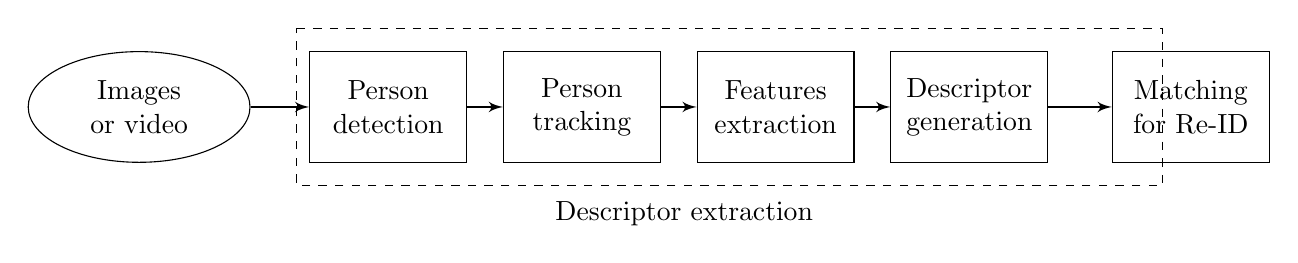
\begin{tikzpicture}
	\node[ellipse, draw, text width=5em, text centered, minimum height=4em](b0){Images or video};
    \node[rectangle, draw, text width=5em, text centered, minimum height=4em, node distance=9em, right of=b0](b1){Person detection};
    \node[rectangle, draw, text width=5em, text centered, minimum height=4em, node distance=7em, right of=b1](b2){Person tracking};
    \node[rectangle, draw, text width=5em, text centered, minimum height=4em, node distance=7em, right of=b2](b3){Features extraction};
    \node[rectangle, draw, text width=5em, text centered, minimum height=4em, node distance=7em, right of=b3](b4){Descriptor generation};
    \path[draw, dashed](2,1)--(13,1)--(13,-1)--(2,-1) node[below=1em, right=9em]{Descriptor extraction} --cycle ;
    \node[rectangle, draw, text width=5em, text centered, minimum height=4em, node distance=8em, right of=b4](b5){Matching for Re-ID};
    \path[draw, -latex', thick](b0)--(b1);
    \path[draw, -latex', thick](b1)--(b2);
    \path[draw, -latex', thick](b2)--(b3);
    \path[draw, -latex', thick](b3)--(b4);
    \path[draw, -latex', thick](b4)--(b5);
	\end{tikzpicture}
\caption{Re-identification system diagram} \label{f1}
\end{figure*}

A typical re-id system performs two basic operations: capturing a unique person descriptor or model and then comparing two models to infer either a match or a non-match. Fig. \ref{f1} shows a schematic representation of a re-id process, detailing subtasks within each component described. The algorithm developed by the authors and presented in this paper has a similar structure as well, whose exact steps will be detailed in subsequent sections.

\subsection*{Project Specifications}
The goal of this project was to develop an application able to identify and recognize subjects, even when they reappear on camera on a later time, using a RGB-D sensor. The functional requirements were:

\begin{enumerate}
\item{dataset creation:}
	\begin{itemize}
	\item{acquisition from RGB-D sensor;}
	\item{manual video tagging and annotation;}
	\end{itemize}
\item{use of a tracking algorithm:}
	\begin{itemize}
	\item{definition of a relevant features set;}
	\item{extract and store features from videos;}
	\end{itemize}
\item{development of a re-identification algorithm that matches a subject against the features dataset.}
\end{enumerate}

The reminder of this paper also follows this structure, and will cover the above items in order: Section \ref{s1} details the creation of the video dataset used to test our re-id algorithm; Section \ref{s3} explains the technical details of the features extraction step; Section \ref{s4} discusses the classification process, commenting on tests and benchmark results; Section \ref{s5} concludes the paper.

\section{DATASET CREATION} \label{s1}
While there is a number of publicly available datasets that are commonly used to test re-id models (ViPER\cite{c2}, ETHZ\cite{c3} and i-LIDS for Re-ID\cite{c4} to name a few), we chose to create one ourselves to be able to use biometric-based features together with the classical appearance-based ones (i.e. colors): the former need to be extracted from the depth data acquired with a RGB-D sensor that none of the aforementioned datasets provide.

In the first phase of our project all groups cooperated to acquire RGB-D videos of 67 people, that were taken using a \emph{Asus Xtion PRO Live} (technical specification are shown in Table \ref{t1}), situated on a ceiling approximately 3.7m tall. The \emph{OpenNI2}\cite{c5} framework was used to acquire the depth data as a fourth video channel (in addition to RGB), containing the point cloud of every frame of the scene. The resulting \texttt{.oni} video files, with a 640x480 resolution and 30fps framerate, are approximately 100MB in size per second.

\begin{figure*}[b] % per fare funzionare "b" serve il pacchetto dblfloatfix
\centering
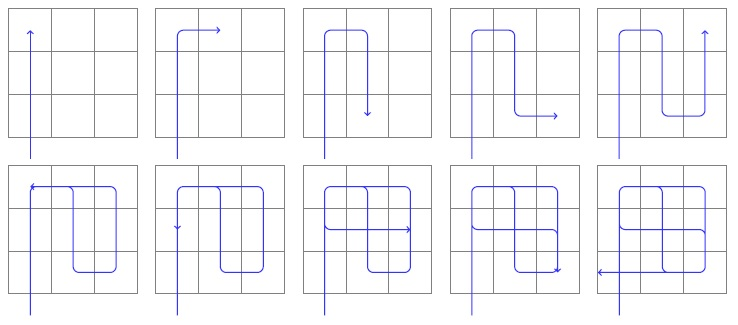
\includegraphics[width=\textwidth]{Percorso.jpg}
\caption{Path followed by subjects in ``single'' videos} \label{f2}
\end{figure*}

This dataset is composed by two different groups of data\cite{c2}\cite{c7}:

\begin{itemize}
\item the first (``single'') consists of 67 top-view videos showing a single person, walking under the camera following the path illustrated in Fig. \ref{f2}: this is done to show each subject from every side. These video are used as a ``training set'' for our application, namely to extract people's features and to generate a knowledge base of features;
\item the second (``group'') consists of 13 top-view videos showing multiple subjects passing one after another under the camera; each one appears two times going in opposite directions and in a different order. These are used as our application's ``test set'', to identify and match instances of people with their extracted features.
\end{itemize}

\begin{table}[h]
\centering
\begin{tabular}{lr}
	\textbf{Power consumption} & below 2.5W\\
	\textbf{Field of view} & 58 H, 45 V, 70 D\\
	\textbf{Sensors} & RGB, Depth, 2x Mic\\
	\textbf{Depth\slash Color image size} & (640x480): 30fps\\
	\textbf{Interface} & USB 2.0\slash 3.0\\
	\textbf{Technology} & Structured light\cite{c6}\\
	\textbf{Operating environment} & indoor\\
	\textbf{Dimensions} & 18 x 3.5 x 5cm\\
\end{tabular}
\caption{Asus Xtion PRO Live datasheet} \label{t1}
\vspace{-1.5em}
\end{table}

Each video was subsequently manually tagged, labeling each training video with a numeric ID corresponding to the subject real name, and each test video with an ID sequence corresponding to the order in which people appeared; the latter acted as a ``ground truth'' to rate the classifier's predicted class against.

\section{FEATURES EXTRACTION} \label{s3}
We developed a script, executable from a Windows, GNU\slash Linux, *BSD and Mac OS terminal, that can both extract subject features and classify people according to its training data (the features set previously saved). Table \ref{t2} details the programming language and libraries used (the listed version numbers correspond to the latest available packages in \emph{Arch Linux} and \emph{AUR} repositories).

\begin{table}[t]
\centering
\begin{tabular}{lr}
	Python & 2.7.10\\
	OpenNI2 & 2.2beta2\\
	OpenCV & 2.4.11\\
	pcl & 1.7.2\\
\end{tabular}
\caption{Libraries used by the application} \label{t2}
\vspace{-1em}
\end{table}

Launching the script with

\begin{center}
\texttt{\$ python2 features.py -f <path>}
\end{center}

triggers the \emph{features extraction} mode: it will open the \texttt{path} video file (must be a \texttt{.oni} video), analyzing both RGB and D channels frame by frame. The features we chose to use for person descriptors and are extracted from videos are:

\begin{itemize}
\item{\emph{height} (mm)}
\item{\emph{head circumference} (px)}
\item{\emph{shoulders circumference} (px)}
\item{\emph{hair color}}
\item{\emph{shirt color}}
\end{itemize}

These features are sampled only in a limited set of frames, in particular the ones in which the person is at the center of the image. We made this choice because while writing code we noticed that depth frames values were skewed due to the camera not being perfectly perpendicular to the floor: the features are extracted only when the subject is within the $11\,$x$\,11$ pixel box centered at $(320,~240)$, in the middle of the video.

Person detection was quite easy to do with the depth cannel info; the only gotcha was to detect and filter pixels with invalid values. After cleaning the frame we segmented the image to create a mask of pixel with values between $a$ and $b$ in Table \ref{t3}, corresponding to white pixels in Fig. \ref{f3}. Setting the $a$ value so high (we lose the subject's shoes) was necessary to filter out the noise caused by the floor.

\begin{table}[b]
\centering
\begin{tabular}{lr}
	a) \textbf{Subject mask (lower bound)} & 150 (mm)\\
	b) \textbf{Subject mask (upper bound)} & 2500 (mm)\\
	c) \textbf{Subject min height} & 1500 (mm)\\
	d) \textbf{Min. shoulders contour area} & 5000 (px)\\
	e) \textbf{Min. head contour area} & 2500 (px)\\
	f) \textbf{Head mask threshold} & 150 (mm)\\
	g) \textbf{Shoulders mask threshold} & 500 (mm)\\
\end{tabular}
\caption{(Arbitrary) thresholds used in our application} \label{t3}
\end{table}

The $c$ threshold in Table \ref{t3} was defined as the minimum height to detect a person in the frame; if the pixel box condition described above is also satisfied the features collection begins:

\begin{itemize}
\item{subject height is calculated as the maximum depth pixels value falling inside the Fig. \ref{f3} mask;
\begin{figure}[t]
	\begin{flushright}
		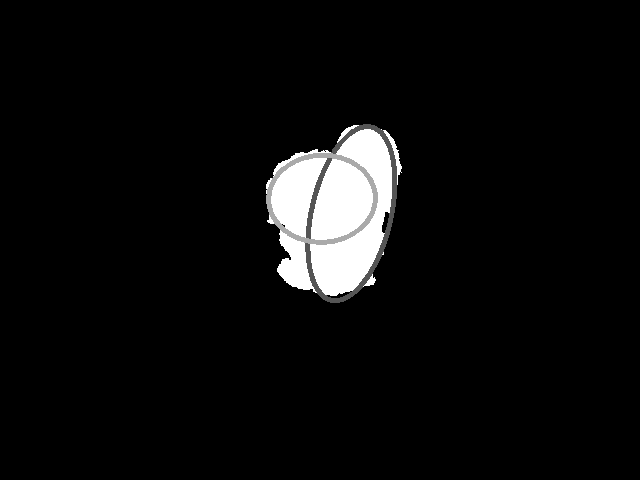
\includegraphics[width=0.4\textwidth]{Mask.png}
		\caption{Subject mask, with head and shoulder area highlighted}
		\label{f3}
	\end{flushright}
\end{figure}}
\item{the depth frame is segmented with a new mask that selects pixels with a value between the extracted height $h$ and $h~-~f$ (in Table \ref{t3}), then the head circumference is calculated with:
\begin{equation}
C_{eq} = \sqrt{4\,\pi A_{eq}} \label{e1}
\end{equation}
where $A_{eq}$ is the area of the mask contour, returned by \emph{OpenCV} function \texttt{cv2.contourArea()}. Shoulders circumference is extracted in the same way, with a mask selecting pixels with values between $h~-~f$ and $h~-~g$ (in Table \ref{t3}) and using (\ref{e1}). In order to get believable values we impose that returned $A_{eq}$ should be higher than $e$ and $d$ (in Table \ref{t3}), for the head and shoulders respectively. Fig. \ref{f3} highlights the fitted ellipses of head and shoulders contours, in light gray and dark gray respectively.}
\item{hair color and shirt color are sampled from the RGB frame with the head and shoulders masks generated on the previous step. Unfortunately, during development we noticed that the color and depth streams are not synced, meaning that applying masks calculated from a depth frame to the corresponding color frame left out a portion of the subject while including a portion of the floor. To get around this, we performed the morphological operation of \emph{erosion} on masks images with a $10\,$x$\,10$ kernel before application. We sample the \emph{dominant} color\cite{c2} as a feature, i.e. the color that appears the most frequently, expressed in the \emph{HSV} colorspace as we found it to be more expressive than \emph{RGB}, in accord with the general results shown in \cite{c9}. Image histogram is calculated with 18 bins for \emph{H} channel and just 4 bins for \emph{S} and \emph{V}, effectively ignoring small color variations.}
\end{itemize}

We take as final features the average reported height and head circumference, the maximum shoulders circumference (because sometimes they are not detected, or only one shoulder is selected), and the most common reported H, S, V values. As a final step, these are normalized according to values in Table \ref{t4}, in order to have the same weight for all the features during the classification process. These values are written in a \texttt{.csv} file, following the subject ID, where every row is a descriptor.

\begin{table}[h]
\centering
\begin{tabular}{lr}
	Height & 2500\\
	Head circ. & 500\\
	Shoulders circ. & 500\\
	H value & 17\\
	S value & 3\\
	V value & 3\\
\end{tabular}
\caption{Normalization values used} \label{t4}
\vspace{-1em}
\end{table}

\addtolength{\textheight}{-6.5cm} % This command serves to balance the column lengths on the last page of the document manually. It shortens the textheight of the last page by a suitable amount. This command does not take effect until the next page so it should come on the page before the last. Make sure that you do not shorten the textheight too much.

\section{CLASSIFICATION} \label{s4}
Launching the aforementioned script with

\begin{center}
\texttt{\$ python2 features.py -k <path>}
\end{center}

triggers the \emph{classification} mode: it will open the \texttt{path} video file (must be a \texttt{.oni} video), extracting subjects features as explained in Section \ref{s3} and matching them with one of the descriptors in \texttt{features\_id.csv}, assigning them an ID.
The chosen classifier is \emph{K-Nearest Neighbor}\cite{c8} as implemented in \emph{OpenCV} (\texttt{cv2.KNearest()}), with $k=1$ so the subject is given the class of their nearest neighbor. We chose K-NN because is one of the simplest and fastest classifying methods, while giving accurate enough results.
The classifier is trained using the already mentioned \texttt{features\_id.csv} as ``training set'' (\texttt{KNearest.train()}), and assigns to new subjects the same class of their \emph{nearest neighbor}, where ``nearest'' means the one with the minimum Euclidean distance, interpreting features descriptors as $n-$dimensional vectors in $\mathbb{R}^n$.

\subsection*{Test results}
We did a little test using a subset of our video dataset, extracting features from 10 ``single'' videos (to use as training set), and successively trying to classify the subjects in 2 of the 13 ``group'' videos (our test set); the subjects in the latter 2 videos are all in the chosen ``single'' videos.
In order to benchmark the algorithm performance we reported the results of the classification on a confusion matrix. Each column of the matrix represents the instances in a predicted class while each row represents the instances in an actual class. Through the confusion matrix, we evaluate the performance of the algorithm defining the following quantities for each subject:

\begin{itemize}
\item{$TP$ (\emph{True Positive}): the number of times the subject has been correctly identified;}
\item{$TN$ (\emph{True Negative}): the number of times other subjects have not been classified as the subject;}
\item{$FN$ (\emph{False Negative}): the number of times the subject has been misclassified as one of the other subjects;}
\item{$FP$ (\emph{False Positive}): the number of times other subjects have been mistakenly classified as the subject;}
\end{itemize}

From the above quantities we derived the following metrics to assess the performance of the classification algorithm:

\begin{itemize}
\item{\emph{Detection Rate} $DR=TP\,\slash\,(TP+FN)$: probability that a subject is classified correctly;}
\item{\emph{False Negative Rate} $FNR=FN\,\slash\,(TP+FN)$: probability that a subject is wrongly classified as one of the other subjects;}
\item{\emph{False Positive Rate} $FPR=FP\,\slash\,(TN+FP)$: probability that other subjects are wrongly classified as the subject;}
\item{\emph{Overall Accuracy} $OA=(TP+TN)\,\slash\,(TP+FP+TN+FN)$: accuracy of the classification algorithm in classifying subjects;}
\end{itemize}

As additional metrics, we calculated the training error executing the script in ``classification mode'' on the ``single'' videos and the script execution times. All the metrics presented above are reported in (\ref{e2}) and tables \ref{t5}, \ref{t6} and \ref{t7}.

\begin{table}[h]
\centering
\begin{tabular}{l|*{10}{c}}
\multicolumn{11}{c}{Predicted class}\\
	& 4 & 5 & 6 & 27 & 28 & 29 & 30 & 31 & 32 & 33\\
	\hline
	4 & 1 & 0 & 1 & 0 & 0 & 0 & 0 & 0 & 0 & 0\\
	5 & 0 & 2 & 0 & 0 & 0 & 0 & 0 & 0 & 0 & 0\\
	6 & 0 & 0 & 1 & 0 & 0 & 0 & 1 & 0 & 0 & 0\\
	27 & 0 & 0 & 0 & 2 & 0 & 0 & 0 & 0 & 0 & 0\\
	28 & 0 & 0 & 0 & 0 & 1 & 0 & 1 & 0 & 0 & 0\\
	29 & 0 & 0 & 0 & 0 & 0 & 0 & 1 & 0 & 1 & 0\\
	30 & 0 & 0 & 0 & 0 & 0 & 0 & 2 & 0 & 0 & 0\\
	31 & 0 & 0 & 0 & 0 & 0 & 0 & 0 & 2 & 0 & 0\\
	32 & 0 & 0 & 0 & 0 & 0 & 0 & 0 & 1 & 1 & 0\\
	33 & 0 & 0 & 0 & 0 & 0 & 0 & 1 & 0 & 0 & 1\\
\end{tabular}
\caption{Confusion matrix for our test} \label{t5}
\end{table}

\begin{equation} \label{e2}
\begin{bmatrix}
	TP & FP\\
	FN & TN\\
\end{bmatrix}
=
\begin{bmatrix}
	13 & 7\\
	7 & 173\\
\end{bmatrix}
\end{equation}

\begin{table}[h]
\centering
\begin{tabular}{lr}
	$DR$ & 65\%\\
	$FNR$ & 35\%\\
	$FPR$ & 3,9\%\\
	\emph{Train. error} & 16,7\%\\
	$OA$ & 93\%\\
\end{tabular}
\caption{Measured performance metrics} \label{t6}
\vspace{-1.5em}
\end{table}

\begin{table}[t]
\centering
\begin{tabular}{lcc}
	& \textbf{``Single''} & \textbf{``Group''}\\
	Avg. time & 15.49s & 33.45s\\
	Min. time & 12.33s & 22.57s\\
	Max. time & 19.44s & 44.33s\\
\end{tabular}
\caption{Test execution timings} \label{t7}
\vspace{-1.5em}
\end{table}

Generally, the most important parameter to evaluate how well an algorithm performs is $OA$, but in this case we consider it not very significant due to high $TN$. For this reason and for the nature of our dataset, the $DR$ is an alternative interesting metric: as showed in Table \ref{t6}, the value of $DR$ is 65\%, which means that our algorithm has a sufficient ability to re-identify people using the 5 features selected. A low $FPR$ means that, for each subject it is quite unlikely that other subjects are classified as they. A 35\% FNR expresses that we should improve the misclassification error. 
Finally a training error of 16,7\% suggests that a better features extraction could be implemented.

\section{CONCLUSIONS} \label{s5}
Our script shows the possibility of re-identify people by means of a fixed set of features, with sufficient performances. To achieve better results, further developments could concern:

\begin{itemize}
\item{adding new features to the subjects descriptor, or improve current features extraction;}
\item{a different classifying algorithm;}
\item{different weights for the features, to give more importance to more relevant or efficient features;}
\item{explore new techniques of features extraction;}
\item{further tweaking of the arbitrary thresholds during mask creation and features detection.}
\end{itemize}

\begin{thebibliography}{9}
\bibitem{c1}P. Tu, G. Doretto, N. Krahnstoever, A.G.A. Perera, F. Wheeler, X. Liu, J. Rittscher, T. Sebastian, T. Yu, K. Harding, \emph{An intelligent video framework for homeland protection}, Proceedings of SPIE Defence and Security Symposium - Unattended Ground, Sea, and Air Sensor Technologies and Applications IX, 2007.
\bibitem{c2}D. Gray, H. Tao, \emph{Viewpoint invariant pedestrian recognition with an ensemble of localized features}, Forsyth, D., Torr, P., Zisserman, A. (eds.) ECCV 2008, Part I. LNCS, vol. 5302, pp. 262–275. Springer, Heidelberg (2008).
\bibitem{c3}A. Ess, B. Leibe, L. Van Gool, \emph{Depth and Appearance for
Mobile Scene Analysis}, Proc. IEEE Int’l Conf. Computer Vision, 2007.
\bibitem{c4}W.-S. Zheng, S. Gong, T. Xiang, \emph{Associating Groups of People}, Proc. British Machine Vision Conf., 2009.
\bibitem{c5}OpenNI2 Downloads and Documentation, \url{http://structure.io/openni}, The Structure Sensor.
\bibitem{c6}B. Freedman, A. Shpunt, M. Machline, Y. Ariel, \emph{US Patent US2010/0118123}, 2010.
\bibitem{c7}W. Zheng, S. Gong, T. Xiang, \emph{Person re-identification by probabilistic relative distance comparison}, Computer Vision and Pattern Recognition (CVPR), 2011 IEEE Conference on. IEEE, 2011, pp. 649–656.
\bibitem{c8}T.M. Cover, P.E. Hart, \emph{Nearest neighbor pattern classification}, IEEE Trans. Inform. Theory, IT-13(1):21–27, 1967.
\bibitem{c9}C. Liu, S. Gong, C.C. Loy, S. Lin, \emph{Person re-identification: what features are important?}, Proceedings of the 12th European conference on Computer Vision, ECCV Workshops, 2012, pp. 391–401.
\end{thebibliography}
\end{document}
